The Figure \ref{fig:dia} presents how the application works.
\newpage
\begin{figure}[H]
	\centering
	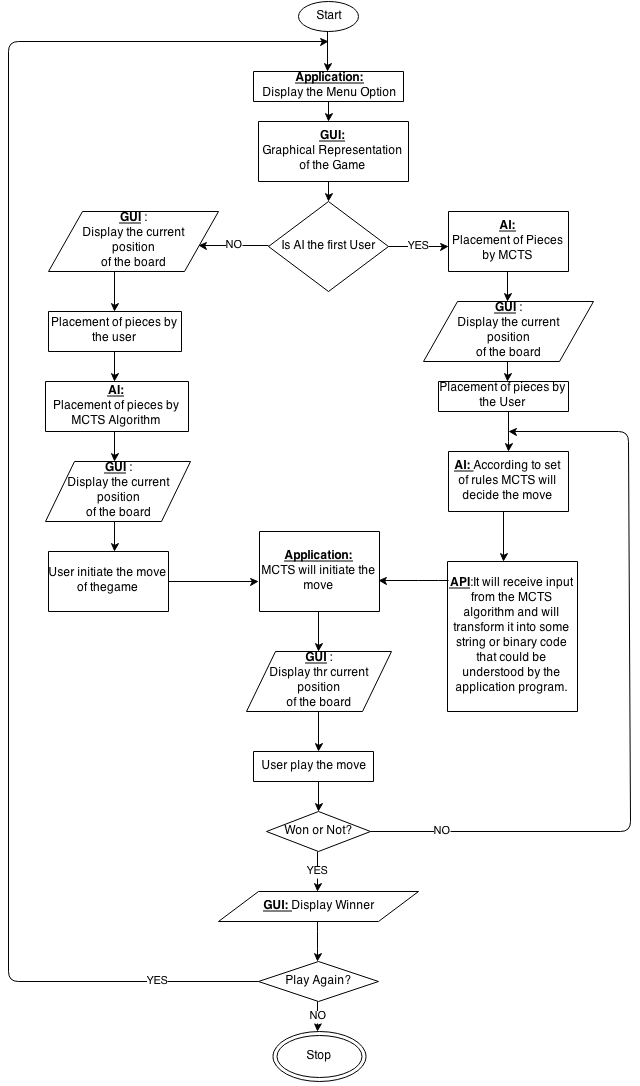
\includegraphics[width=0.80\textwidth]{2General_Architecture/2.1.2GeneralView/api.png}
	\caption{The flowchart describing the usage of the API}
	\label{fig:dia}
\end{figure}
\thispagestyle{empty}

First, the menu displays. Then, the players place their pieces, and they play. It is possible to see which module interacts with each other. To go deeper, the four modules will be presented in Figure \ref{fig:gra}.

\begin{figure}[!h]
\centering
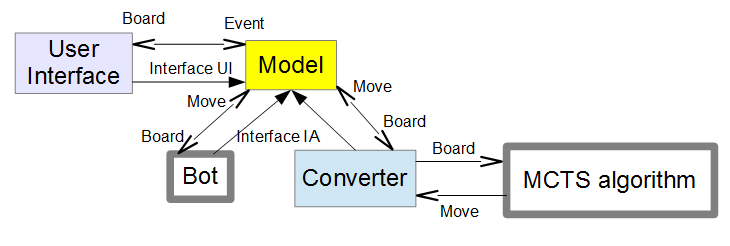
\includegraphics[width=1\textwidth]{2General_Architecture/2.1.2GeneralView/prep.png}
\caption{General view of the architecture}
\label{fig:gra}
\end{figure}

The 4 modules and the Bot will be described :

\begin{itemize}
\item \textbf{User Interface module}

This module will communicate with the environnement, displaying the board, creating events, like mouse clics and keyboard events. Then it will send them to the Model module. The User Interface is studied more deeply in part \ref{sec:ui}. An interface is used to make it possible for the future user of our project to replace this User Interface by his own, just by implementing an interface.

\item \textbf{Model module}

This module will handle the game itself. It will be able to store and play games, receiving moves and giving the state of the board to the User Interface and the AI. A type Move will be created, to impose the move format. The Model module contains as well the rules of the game. It is the link between the user and the IA.

\item \textbf{Converter module}

This module is the link between the Model module and our IA, the MCTS algorithm. It forwards the board sent by the Model module to the MCTS algorithm, adapting the format. Furthermore, it does the same communication in the other way with the final move, from the MCTS algorithm to the Model module with the adapted format. The Converter module is described in part \ref{sec:api}.

\item \textbf{The MCTS Algorithm module}

This module is the Artificial Intelligence of our project. Giving a board by the Converter module, it is able to send back the move. The MCTS algorithm module is defined in the part \ref{sec:mctss}.

\item \textbf{Bot}
A Bot is an Artificial Intelligence as well. Our work will make possible the adding of other IA, or Bots, conceived by everyone, just by implementing the AI interface. For instance, there are some free bots already available on the site \textit{Arimaa.com}.
\end{itemize}